\documentclass{article}

\usepackage{graphicx}
\usepackage{tikz}
\usepackage{tikzsymbols}
\usetikzlibrary{calc,patterns,shapes.geometric}
\pagestyle{empty}
\usepackage[margin=0pt]{geometry}
\geometry{papersize={14in,12in}}

\def\centerarc[#1](#2)(#3:#4:#5){\draw[#1] ($(#2)+({#5*cos(#3)},{#5*sin(#3)})$) arc (#3:#4:#5);}

\begin{document}
	\begin{figure}
		\centering
		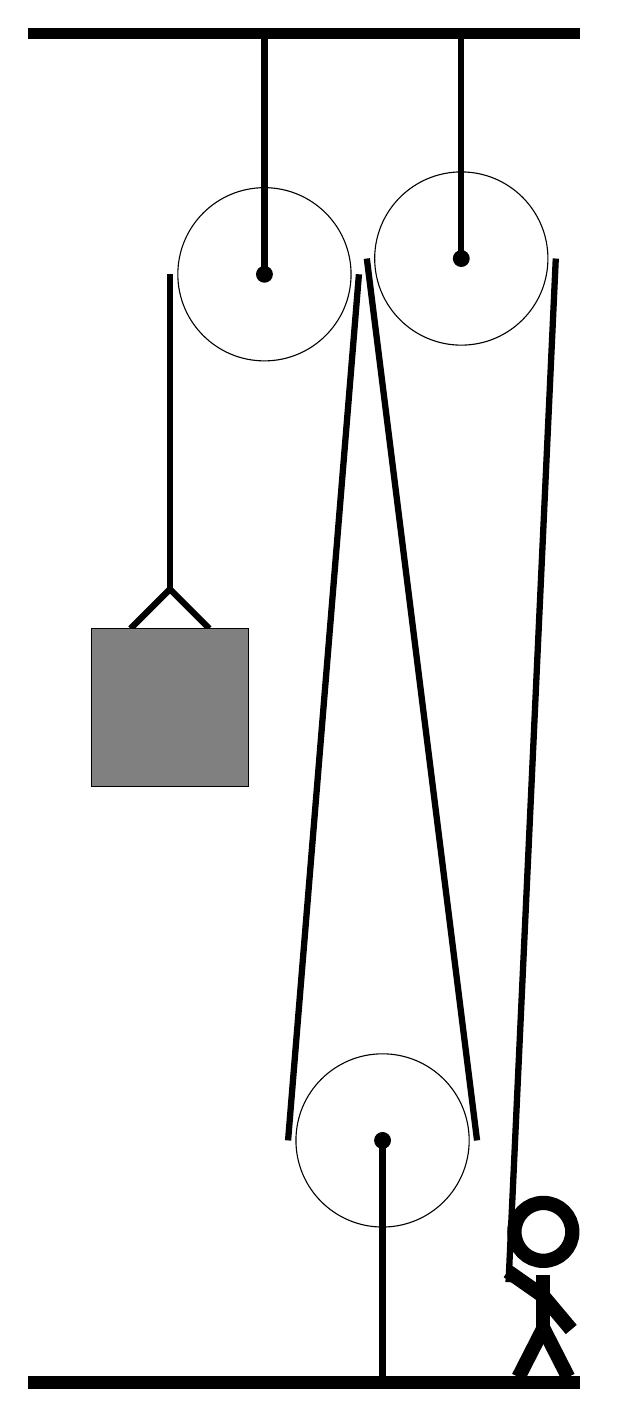
\begin{tikzpicture}
			%%%%% START %%%%%
			\draw[fill=black] (-2, 14) rectangle (5, 14.125);
			
			\draw (1, 11) circle (1.1);
			\draw[fill=black] (1, 11) circle (0.1);
			\draw[line width=0.8mm]  (1, 14) -- (1, 11);
			
			\draw[fill=white](2.5, 0) circle (1.1);
			\draw[fill=black] (2.5, 0) circle (0.1);
			\draw[line width=0.8mm]  (2.5, -3) -- (2.5, 0);
			
			\draw[fill=white](3.5, 11.2) circle (1.1);
			\draw[fill=black] (3.5, 11.2) circle (0.1);
			\draw[line width=0.8mm] (3.5, 14) -- (3.5, 11.2);
			
			\draw[line width=0.8mm] (-0.7, 6.5) -- (-0.2, 7.0) -- (0.3, 6.5);
			\draw[fill=black!50] (-1.2, 6.5) rectangle (0.8, 4.5);
			
			\draw[line width=0.8mm] (-0.2, 11) -- (-0.2, 7.0);
			\centerarc[line width=0.8mm](1, 11)(0:180:1.2000000000000002);
			\draw[line width=0.8mm](2.2, 11) -- (1.3, 0);
			\centerarc[line width=0.8mm](2.5, 0)(180:360:1.2000000000000002);
			\draw[line width=0.8mm](3.7, 0) -- (2.3, 11.2);
			\centerarc[line width=0.8mm](3.5, 11.2)(0:180:1.2000000000000002);
			\draw[line width=0.8mm](4.7, 11.2) -- (4.1, -1.8);
			
			\node at (4.5, -1.9) {\Strichmaxerl[10][-35][-50]};
			
			\draw[fill=black] (-2, -3) rectangle (5, -3.15);
			%%%%% END %%%%%
		\end{tikzpicture}
	\end{figure}	
\end{document}